\section{Organic traffic control}

\subsection{What is Organic Traffic Control (OTC)}

Organic Traffic Control is a system to decrease the waiting time and fuel consumption at
intersections with traffic lights in urban areas. To accomplish this goal the system optimises the
signal times with the help of data gathered locally.

To accomplish this goal the first organic traffic control system presented in this paper uses a layered system. Three layers control the signal plan at the intersection, gather data about waiting times to change the signal plan if needed and adapt to situations which are not sufficiently covered by existing signal plans. Changes can be introduced in run-time because the layers split the tasks into an online component able to change the signal plans quickly to react to current traffic demand and an offline component which executes the more time consuming tasks.  Theses layers are further explained in section B.

In section C an experiment using this organic traffic control method is presented which was based on two real intersections modelled in software with section D explaining the results of the experiment.

Section E presents a further development based on the OTC to combine intersections optimised by a OTC system to allow combined intersections improve traffic flow even more

\subsection{Layers of Organic Traffic Control}
Layer 0
 is not part of the OTC system but is needed for the organic Layers 1 and 2. It is used to control the traffic with a Traffic Light Controller which is either implemented as a FTC or a traffic responsive controller which is able to switch phase durations. These changes of the traffic responsive controller are used to manage small variations in traffic demand and are based on data gathered by detectors at the intersections. Implementing a FTC is easier but makes it necessary to change the signal plans more often. In general the signal plan used should optimise the waiting times at the intersection for the current traffic situation.
 
 Layer 0 is needed at every intersection and guarantees that the traffic lights are always functioning even if the organic component should not be available due to maintenance or system errors. \cite{organic1}\cite{organicLCS}\ \\
 
Layer 1
the online component of the OTC system is monitoring the traffic to switch the signal plans of Layer 0 if changes in the traffic occur which lead to increasing waiting times. Layer 1 uses detectors available at Layer 0 to collect these information. From the gathered data Layer 1 creates vectors for each turning at the intersection containing vehicles per hour. These vectors are used to determine important turnings at the intersections and as input for a Learning Classifier System (LCS) which is used to determine the change of signal plans.[5]

A LCS is a system that uses different rules to respond to situations and evaluates the rules to learn the best response to different inputs. Theses rules are called classifiers and consist of three parts: condition, action and evaluation. The condition is used to determine for which input the classifier is usable. If the condition is met and a classifier is usable the action defines what the classifier would do in this situation. In the case of OTC the action is the signal plan that Layer 1 determines for the TLC of Layer 0 to use with current traffic. Lastly the evaluation is used to provide feedback on how well the classifier would perform in the current conditions. Selecting a classifier is done in two steps. First all classifiers that are suitable for the present input are combine into the so called \textit{match set}. After that the actions of all classifiers in the \textit{match set} are compared and the one with the best evaluation is used. If two or more classifiers want to use the same action the average evaluation of these classifiers is used to determine if the action has the best evaluation. The classifiers recommending the best action form the \textit{action set} and their evaluation is later updated with the feedback gathered in the real environment. In the case of OTC the feedback from the real environment are the waiting time of vehicles and the amount of vehicles at the intersection.\cite{organic1}\cite{organicLCS}

Layer 1 can perform well with using LCS as long as there are applicable classifiers for every input at the intersection. Normally if a situation occurs which is not covered sufficiently by the available classifiers a new one is generated using a random action, default evaluation and a matching condition of the available classifiers. This approach however is not useful for traffic control as applying a random action i.e. a random signal plan would in most cases lead to increasing waiting times. Therefore Layer 2 is used to create and test new classifiers before using them on Layer 1. \cite{organic1}\cite{organicLCS}

As this system has a low demand for computing power it can be installed locally at every intersection.\cite{organicLCS}\ \\

Layer 2 the offline component of the OTC system creates new classifiers for the implementation in Layer 1. In case of traffic control this means that the TLC gets new signal plans as a result of the actions of the new classifiers. An evolutionary algorithm creates these new classifiers and afterwards a traffic simulation software tests and evaluates the new signal plans. 
Testing the signal plans of the new classifiers before the implementation in Layer 1 guarantees that bad or unsafe plans are not used at the real intersection. It also provides an approximated quality for the signal plan. Even tough the process of creating and evaluating a new classifier is faster in a simulated environment than it would be at a real intersection the results might not be available for Layer 1 to react on an immediate change of traffic. In this case the classifier which condition is closest to the current input is used and the condition extended to apply to the current input. This ensures that Layer 1 is able to react immediately and still perform acceptable.\cite{organic1}\cite{organicLCS}

Using a traffic simulation for Layer 2 requires a higher demand of computing power than Layer 1
needs. This means that Layer 2 may not be locally at every intersection but instead central and in use for a group of intersection. As Layer 2 is only used when a traffic situations occurs at one of the intersections which is not optimal covered by existing classifiers and therefore is not always needed at every intersection there is no problem with using Layer 2 for a couple of intersections.\cite{organicLCS}

\subsection{Experimental setup for intersections}
The OTC approach was tested in an experiment to compare the waiting time of vehicles at two intersections between the OTC and a normal FTC. As models for the experiments two existing intersections K7 and K3 both located in Hamburg Germany were simulated using a traffic
simulation software.

As seen in Fig. \ref{fig:K7} K7 is a three armed intersection with six turning manoeuvres  while in Fig. \ref{fig:K3} K3 is shown having four arms and eleven turning manoeuvres. Both intersections have a traffic peak between 8:00 am and 9:00 am in the morning. This allows to test the impact on waiting times when traffic demand is increasing rapidly in a short amount of time between the OTC and FTC. The traffic at both intersections is modelled after a traffic census carried out by the local authorities.\cite{organic1}

\begin{figure} [!htb]
	\centering
	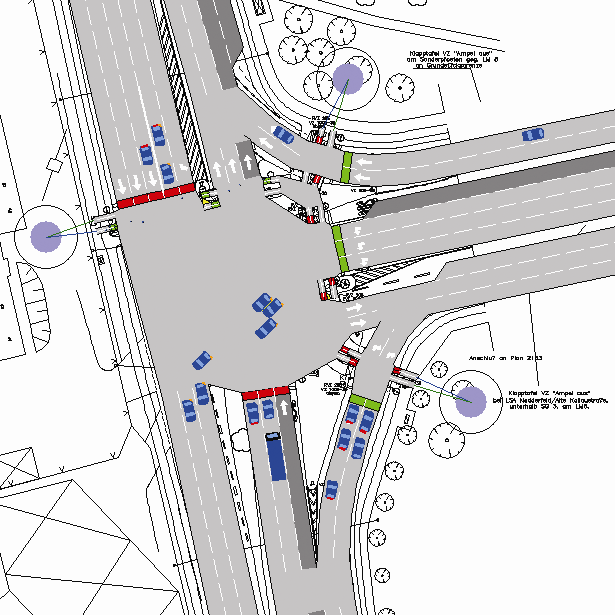
\includegraphics[scale=0.45]{pic/K7.png}
	\caption{K7 \cite{organic1}}
	\label{fig:K7}
\end{figure}

\begin{figure} [!htb]
	\centering
	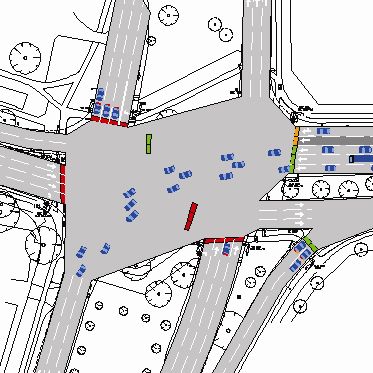
\includegraphics[scale=0.70]{pic/K3.png}
	\caption{K3 \cite{organic1}}
	\label{fig:K3}
\end{figure}

At both intersections the experiments use a six hour time frame starting at 6:00 am with low traffic demand. As mentioned above the traffic peak is reached between 8:00 am and 9:00 am. Afterwards the traffic is remaining steady on a medium level during the rest of the experiments. Throughout the entire time a traffic simulation software is used to calculate the average delay at both intersections as well as to calculate the effectiveness of new signal plans create by Layer 2 of the OTC. This average waiting value is used to compare the results of the OTC and FTC.\cite{organic1}

The OTC experiments were simulated for three consecutive days to test the learning capabilities of the organic approach. At the beginning of Day 1 the set of classifiers for the LCS of Layer 1 is empty. Layer 2 is used to create new classifiers for Layer 1 which are afterwards available for the rest of the experiment. Each of the three days was simulated at least three times.\cite{organic1}


\subsection{Results for K7 and K3}
The results compared in this section are based on the average delay measured during the experiments and compares the different days of the OTC approach with each other and the FTC.\ \\

K7 Results: At the beginning of Day 1 the OTC approach is performing worse than the FTC as seen in Fig. \ref{fig:K7result} because Layer 1 has no adapted classifiers available. The OTC is able to improve quickly and is outperforming the FTC even before the morning traffic peak. Throughout the rest of the experiment the OTC approach is consistently performing better than the FTC. During the increasing traffic demand at the morning peak Layer 2 is used frequently to create new classifiers for the latest input. Classifiers used during this time by Layer 1 often do not meet the conditions of the current traffic but are widened and used until Layer 2 has created applicable classifiers. Over the entire first day the OTC performs on average 10 \% better.\cite{organic1}

On Day2 and Day3 the OTC is able to outperform the FTC over the entire experiment. As Layer 1 has already stored the classifiers used on the previous days Layer 2 is used less often than on Day1 and solutions for the input on Layer 1 are often available immediately. Overall the average delay is reduced by about 12\%.\cite{organic1}\ \\

\begin{figure} [!htb]
	\centering
	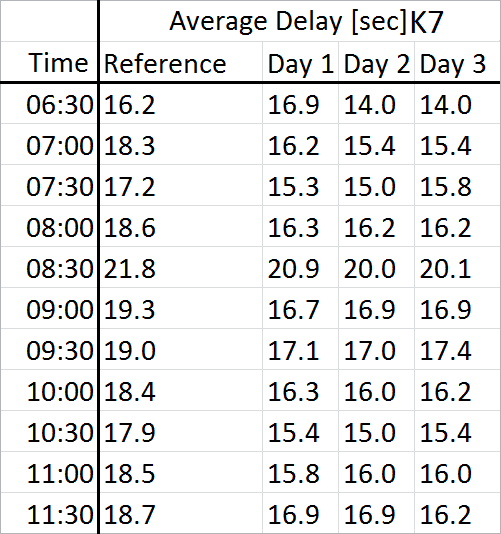
\includegraphics[scale=0.60]{pic/K7_ResultTable.png}
	\caption{Results of K7. Table created from graph used for the results of K7 \cite{organic1}}
	\label{fig:K7result}
\end{figure}

K3 Results: Overall the Results for K3 shown in Fig. \ref{fig:K3result} are similar to the ones of K7. The average delay is higher for the FTC as well as the OTC approach but even with the empty classifier set at the beginning of Day 1 the OTC approach is able to perform around 6\% better than the FTC on the first day. For Day2 and Day3 the classifier set is containing the classifiers of the previous days allowing to handle especially the morning peak better than the FTC. Overall the average improvement is around 8\%.\cite{organic1}\ \\

The experiment results of K7 and K3 indicate that it is possible to decrease waiting time at intersections using a OTC which is also able to adapt to change in traffic demand.

\begin{figure} [!htb]
	\centering
	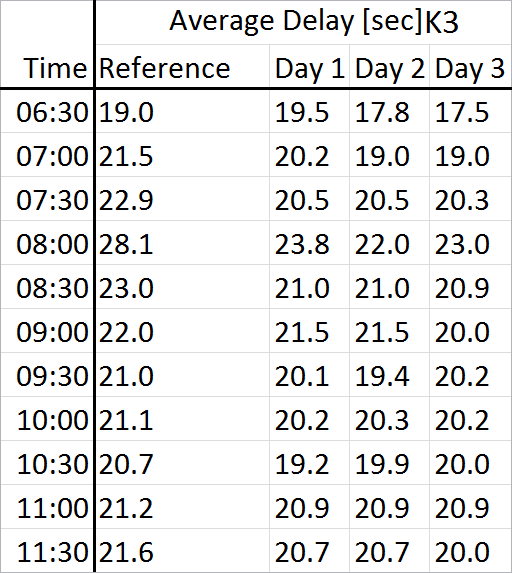
\includegraphics[scale=0.60]{pic/K3_ResultTable.png}
	\caption{Results of K3. Table created from graph used for the results of K3 \cite{organic1}}
	\label{fig:K3result}
\end{figure}

\subsection{Distributed progressive signal systems}
The OTC system presented so far is optimising traffic at one intersection in an urban road network. If this system is installed at most of the intersections in the area they are all locally optimised but do not communicate with each other. This may again lead to longer waiting times as vehicles have to pass multiple intersections which are not coordinated.\cite{organic1}\cite{organicRouting}

The idea of distributed progressive signal systems (DPSS) is to find network nodes which form partnerships in a first step.  All nodes in a partnership then agree on using the same cycle times to synchronise the traffic flow in the second step. Lastly in the third step all nodes choose TLCs considering the agreed cycle time and finally calculate the offsets to each other. These three steps will now be described in detail.\ \\

First Step: All nodes analyse which of their turnings has the strongest traffic flow. Then each node informs its neighbouring nodes about whom they would like as successor and predecessor. As an example Fig. \ref{fig:flow} can be used: Both nodes in the middle of the road network shown in the graphic have determined the dark blue downward pointing arrow as their strongest traffic flow. As a result they inform the upstream node that they would like them as predecessor and the downstream node to be their successor.

\begin{figure} [!htb]
	\centering
	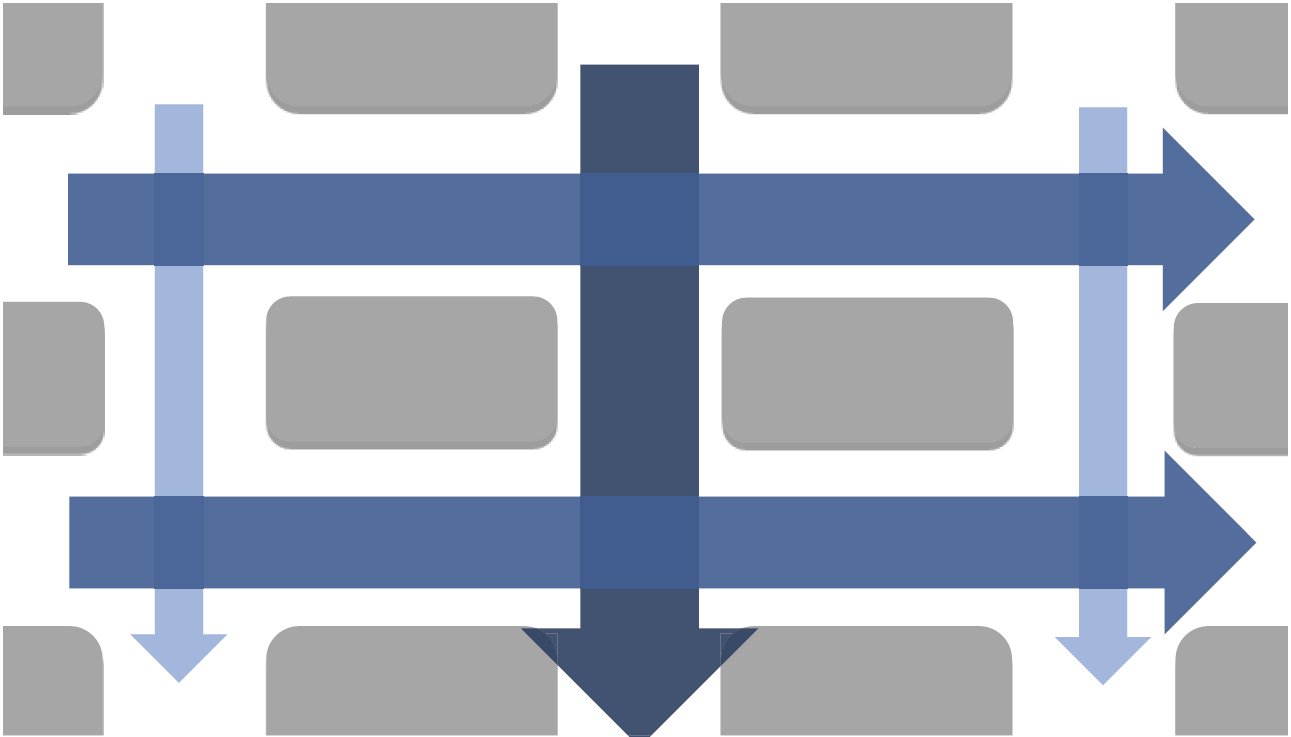
\includegraphics[scale=0.25]{pic/TrafficFlow.png}
	\caption{Traffic flow \cite{organicHPSS}}
	\label{fig:flow}
\end{figure}

When all nodes have determined their predecessors and successors a matching takes place to build groups of nodes. After the matching all nodes check whether they were chosen by their downstream node as predecessor and accept the partnership if this is the case. Remaining nodes which did not get their desired predecessor receive a message and can try to find a partnership with their second strongest stream. As all nodes participating in a DPSS get a message from their predecessor and their successor every node knows its direct partners.\cite{organic1}\ \\
Second Step: The nodes in a partnership now try to find a common cycle time which needs to be long enough for the nodes with the strongest traffic demand to allow fluent traffic flow and still be as short as possible so that nodes with lower traffic flow do not suffer from the longer waiting times for their vehicles.
To find the common cycle time each node first decides on his own \textit{desired cycle time}. It is chosen for the case that the node is not part of a DPSS using the LCS of Layer 1. Normally the LCS chooses a signal plan that has optimised cycle times for the node which means they are short enough to minimize the waiting times of all vehicles.
When all nodes have found their \textit{desired cycle time} the longest of these is chosen as the \textit{agreed cycle time} (ACT). This way the ACT ensures the best traffic flow at the nodes with the highest traffic demand and keeps the waiting times at other nodes as short as possible. A longer cycle time increases the average waiting times for vehicles because the green phase for each turning is longer than needed for all vehicles to pass the intersection. After all waiting vehicles have passed the throughput for the turning decrease while other turnings still have waiting vehicles. \cite{organic1}\ \\
Third Step: When all nodes are informed about the ACT each node can locally choose a TLC suitable for the cycle time. Afterwards the nodes need to determine their offset to allow the synchronisation of the nodes. This is needed so that vehicles starting at the first node of the DPSS have to stop as little as possible while following nodes of the DPSS. Important factors for the synchronisation are the offset of the predecessor, the time vehicles need to travel from the predecessor and the time needed at the node for all already waiting vehicles to leave the node.\cite{organic1}\ \\

Integration of DPSS in existing OTCs: With some small adjustments it is possible to integrate DPSS into existing OTCs. Primarily the LCS of Layer 1 has to be updated to work with the additional restrictions of DPSS especially the changes to cycle times. In the beginning the LCS tries to find classifiers who implement the ACT and meet the current conditions at the intersection. In the case that none such classifier could be found the LCS changes one of the existing classifiers to match the ACT. This new classifier is included into to the available set of classifiers.\cite{organic1}\ \\

Comparing OTC with OTC-DPSS: An experiment was conducted to study possible improvements of the OTC-DPSS approach over the simple OTC approach. Two different scenarios were used for the experiment. The first model was an arterial road with five intersections in a row while the second used a Manhatten network with a total of six intersections in two rows. In both scenarios the intersections had a distance of 250m to each other.

To research possible improvements both the OTC and the OTC-DPSS system were compared in regards to the average delay at the intersections, the average time vehicles spent traveling through the entire network and the average amount of stops vehicles had to do in the network.\cite{organic1}\ \\

Results: For the arterial road it was possible to decrease the average amount of stops during nearly the entire experiment. Overall the decrease in stops was around 15\% while the average travel time could not be improved significantly. For the OTC-DPSS approach the average delay was quite different for the individual nodes. The nodes in the middle profited from the DPSS and had lower waiting times than they had in the OTC system. In contrast the first node of the DPSS had increased waiting times as the node did not profit from the synchronisation of DPSS.

For the Manhatten network several DPSS were created during the experiment for different intersections. Similar to the results of the arterial road it was not possible to significantly reduce the travel time in the network but the amount of stops could be decreased by around 7\%.\cite{organic1}

The aterial road as well as the Manhatten network were improved by the implementation of the OTC-DPSS over the use of only the OTC especially regarding the number of stops in the networks.

% {\ss} 
% \"u